%CP_prerequisite_relation

\documentclass[problem]{mcs}

\begin{pcomments}
  \pcomment{from: S09.cp3r}
  \pcomment{There is some pdf error that needs to be addressed}
%  \pcomment{}
\end{pcomments}

\pkeywords{
  relations
  scheduling
  partial_orders
}

%%%%%%%%%%%%%%%%%%%%%%%%%%%%%%%%%%%%%%%%%%%%%%%%%%%%%%%%%%%%%%%%%%%%%
% Problem starts here
%%%%%%%%%%%%%%%%%%%%%%%%%%%%%%%%%%%%%%%%%%%%%%%%%%%%%%%%%%%%%%%%%%%%%

\begin{problem} \mbox{}  %LaTeX artifact to position the table

\begin{center}
\begin{tabular}{|l|l|}
\hline
Direct Prerequisites & Subject\\ \hline
 18.01 & 6.042\\ \hline
 18.01 & 18.02\\ \hline
 18.01 & 18.03\\ \hline
 8.01  & 8.02\\ \hline
 8.01  & 6.01\\ \hline
 6.042 & 6.046\\ \hline
 18.02, 18.03, 8.02, 6.01 & 6.02\\ \hline
 6.01, 6.042 & 6.006\\ \hline
 6.01 & 6.034\\ \hline
 6.02 & 6.004\\ \hline
\end{tabular}
\end{center}

\bparts

\ppart\label{prereqtable} For the above table of MIT subject
prerequisites, draw a diagram showing the subject numbers with a line
going down from each subject to each of its (direct) prerequisites.

\begin{solution}
%\TBA{pdf bug in figure}
\textbf{TBA}

\iffalse
\begin{center}%causes latex error
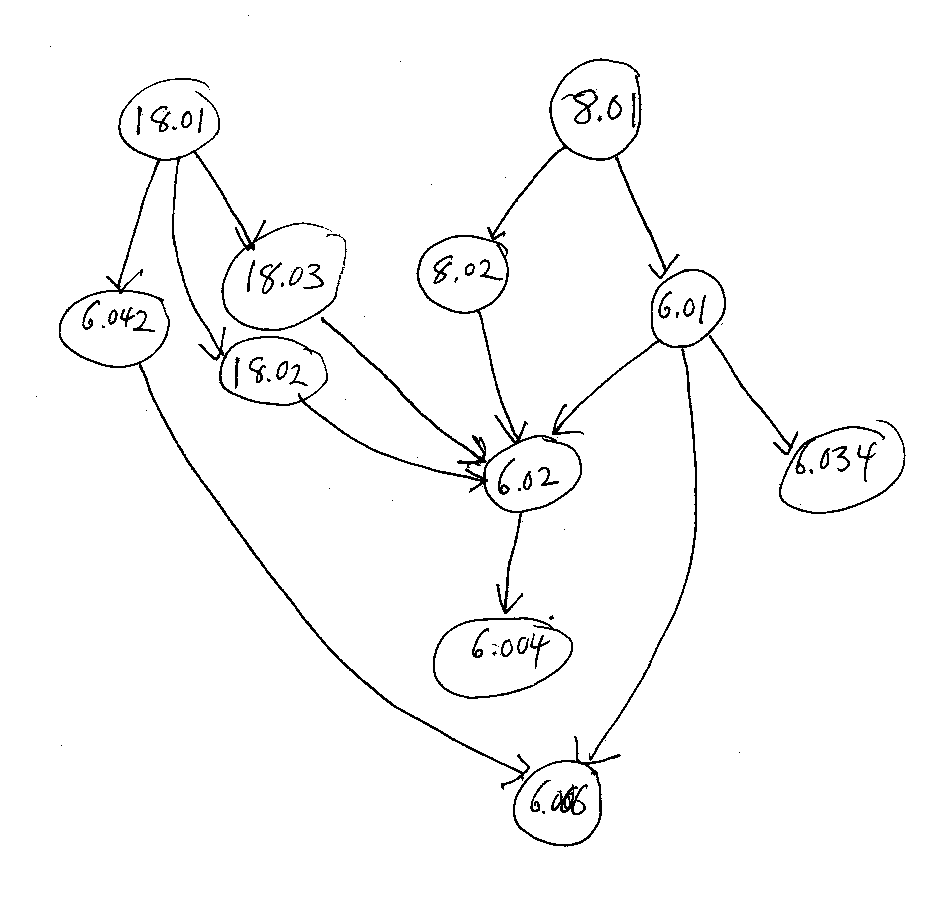
\includegraphics[height=2.5in]{prereq-poset}%.pdf}
\end{center}
\fi

\end{solution}

\eparts

For each of the following binary relations, describe an isomorphic (``same
shape'') collection of sets partially ordered by the proper subset
relation, $\subset$.

\bparts

\ppart The prerequisite relation among MIT subjects from part\eqref{prereqtable}.
Explain what would go wrong if the set corresponding to a subject consisted only
of its indirect prerequisites (that is, the subject itself was not
included in the corresponding set)?  \hint Consider 18.01 and 6.042.

\begin{solution}
  For each subject, let the corresponding set be the subject itself along
  with all the subjects that are indirect prerequisites of that subject.
  (Remember that a direct prerequisite is considered to be a special case
  of an indirect one.)  For example, the set corresponding to 6.006 would
  be $\set{\text{6.006, 6.01, 6.042, 18.01}}$.

If the subject itself was not included in its corresponding set, then
subjects like 18.01 and 6.042 that have the same prerequisites would both
correspond to the same set, so the correspondence between subjects and
sets would not be a bijection.
\end{solution}

\ppart  The ``empty'' relation on 5 elements.  That is, the relation
under which no element is related to anything.

\begin{solution}
  Letting the five elements be $1,2,3,4,5$, the recipe of mapping an
  element to its preimages under the relation, with the element itself
  thrown in, gives the five sets $\set{1},\set{2},\set{3},\set{4},\set{5}$.

Of course any 5 sets none of which is contained in any of the others will
also work, for example, all the size 4 subsets of $\set{1,2,3,4,5}$

\textbf{Quick Question}: The empty binary relation on a set is defined to
be the relation whose graph is empty, that is, it has no arrows.  Why is
the empty relation a strict partial order?  Why isn't it a weak partial
order?

\iffalse
It's vacuously asymmetric and transitive.  It's not reflexive because
element don't have self-looping arrows.
\fi

\end{solution}

\ppart The "properly contains'' relation, $\supset$, on
$\power{\set{1, 2, 3,4}}$.

\begin{solution}
  The standard inverse image solution involves sets of subsets.  A more
  elegant correspondence is to let each set $A \subseteq \set{1, 2, 3,4}$
  correspond to its complement.  That is,
\[
f(A) = \bar{A} \eqdef \set{1, 2, 3,4} - A.
\]
This works because $A \supset B$ iff $\bar{A} \subset \bar{B}$
\end{solution}

\eparts

\end{problem}

%%%%%%%%%%%%%%%%%%%%%%%%%%%%%%%%%%%%%%%%%%%%%%%%%%%%%%%%%%%%%%%%%%%%%
% Problem ends here
%%%%%%%%%%%%%%%%%%%%%%%%%%%%%%%%%%%%%%%%%%%%%%%%%%%%%%%%%%%%%%%%%%%%%

\endinput
